\subsection{Geometry, not lead count}
On the PTB-XL QRS dipolar subspace, the closed-form gain $\kappa_s(S)$ ranks
configurations by \emph{conditioning}, not lead count: a single Lead~I observes only
one of three dipole directions (rank 1); a spread triplet $\{$I,\,II,\,V2$\}$ gives
$\kappa{=}\kapSpan$; three adjacent precordials $\{$V1,\,V2,\,V3$\}$ give
$\kappa{=}\kapColl$; but three \emph{coplanar} limb leads $\{$I,\,II,\,III$\}$ give
$\kappa{=}\kapCopl$ and the six limb leads $\kappa{=}\kapLimb$---so six frontal-plane
leads recover the (transverse) dipole far worse than three well-chosen ones.

\subsection{RMSE hides fabrication; the certificate reveals it}
Table~\ref{tab:hall} reconstructs the unobserved leads from $\{$I,\,II,\,V2$\}$ with
three methods. Their per-lead RMSE is nearly identical, yet the certificate separates
them. The dipolar baseline places \emph{zero} energy in the certified-unrecoverable
subspace ($h{=}0$): it never fabricates, but recovers only Tier~I. The learned linear
(OLS) reconstructor places moderate energy there that is \emph{positively correlated}
with the true non-dipolar content (it genuinely recovers Tier~II). The generative
reconstructor places the \emph{most} energy there, but that energy is
\emph{uncorrelated with truth} (correlation $\approx\genCorr$)---confident
fabrication that RMSE cannot detect and the certificate flags. The pattern is
identical across the Lead-I and limb-6 configurations (see \texttt{results/}).

\begin{table}[t]
\centering
\caption{Reconstruction from $\{$I,\,II,\,V2$\}$ on PTB-XL (fold 10). RMSE is matched;
the certificate's hallucination energy $h$ (mV) and non-dipolar correlation
$\rho$ with truth are not. Generative energy is uncorrelated with truth.}
\label{tab:hall}
\small
\begin{tabular}{llccc}
\toprule
seg & method & RMSE\,(mV) & $h$\,(mV) & $\rho$ \\
\midrule
\multirow{3}{*}{QRS}
 & dipolar     & 0.196 & 0.000 & $+0.00$ \\
 & OLS         & 0.196 & 0.030 & $+0.13$ \\
 & generative  & 0.228 & 0.097 & $+0.00$ \\
\midrule
\multirow{3}{*}{ST}
 & dipolar     & 0.125 & 0.000 & $+0.00$ \\
 & OLS         & 0.112 & 0.016 & $+0.28$ \\
 & generative  & 0.149 & 0.063 & $-0.00$ \\
\midrule
\multirow{3}{*}{T}
 & dipolar     & 0.140 & 0.000 & $+0.00$ \\
 & OLS         & 0.105 & 0.028 & $+0.44$ \\
 & generative  & 0.163 & 0.067 & $-0.00$ \\
\bottomrule
\end{tabular}
\end{table}

\begin{figure}[t]
  \centering
  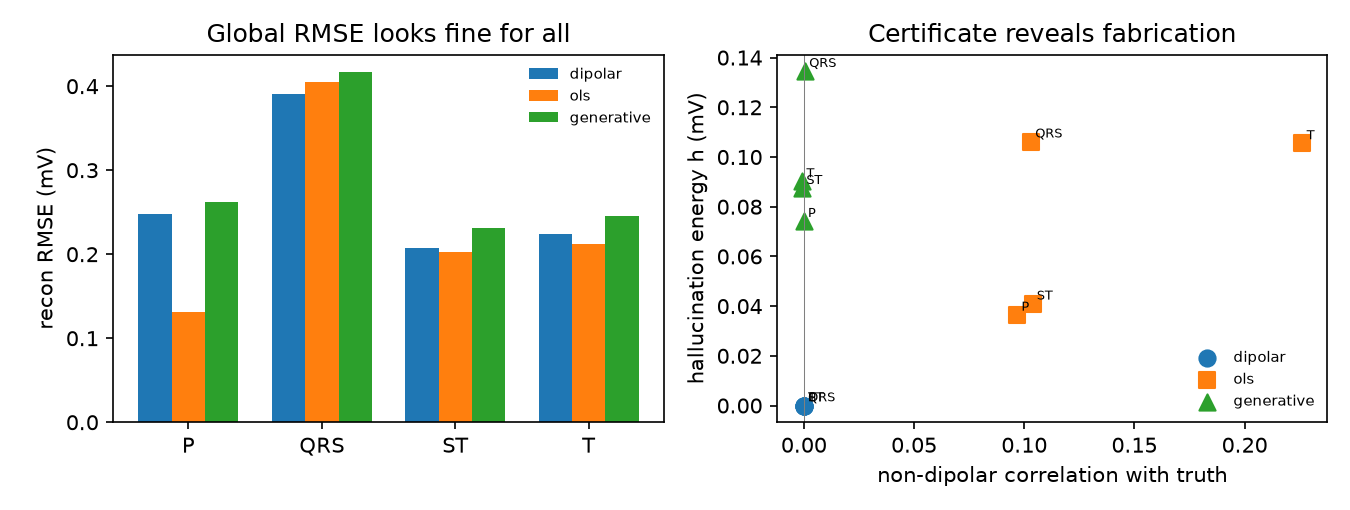
\includegraphics[width=\linewidth]{../results/ptbxl_hallucination.png}
  \caption{Left: global RMSE is similar for all reconstructors (limb-6$\to$precordial).
  Right: in the hallucination-energy vs.\ non-dipolar-correlation plane the generative
  model sits at high $h$, near-zero correlation---fabrication the certificate isolates.}
  \label{fig:ptbxl}
\end{figure}

\subsection{Safety case: precordial ST from limb leads}
The certificate warns \emph{before} reconstruction that limb-6$\to$precordial is
unsafe for an ST decision: $\kappa{=}\kapLimb$ and the ST segment is only $\dipST$
dipolar, so precordial ST is largely Tier~III. The danger is real and
\emph{bidirectional}. Over $799$ fold-10 records, measuring ST deviation (J$+$60\,ms
vs.\ the PR baseline, $0.1$\,mV threshold) on true vs.\ reconstructed V1--V6, the
generative reconstructor \emph{fabricates} $263$ phantom STEMIs (true signal negative),
whereas the conservative OLS reconstructor \emph{masks} $360$ real ones---opposite,
both-dangerous failures, at an identical $\sim\!0.075$\,mV mean ST error that RMSE
cannot separate. The per-reconstruction flag catches \emph{fabrication} (it detects
added, not missing, energy), abstaining on the highest-$h$ generative ST segments at a
controlled rate; masking is a property of the configuration, which the certificate's
$\kappa$ flags upfront. The lesson is the certificate's, not a single reconstructor's:
this configuration should not drive a precordial ST call. Counts in
\texttt{results/ptbxl\_stemi.json}.

\subsection{Guarantees under device shift}
Calibrating on the Schiller CS device family and testing on the AT family (a genuine
within-PTB-XL device shift), the ST/V4 interval keeps nominal $0.90$ coverage
in-distribution but drops to $0.82$ on the shifted device under plain conformal.
Weighted conformal \cite{tibshirani2019weighted} restores coverage (conservatively, to
$1.00$) and a $300$-record slice recalibration returns it to $0.93$
(\texttt{results/cross\_device.json}). Tier~I exactness and the Tier~III flag's
soundness are unaffected, as promised: only the Tier~II \emph{level} is shift-sensitive,
and it is both measurable and repairable.

